\documentclass[11pt]{article}
% Shared article typography. Build with pdfLaTeX.
\usepackage[left=0.85in,right=0.85in,top=0.80in,bottom=0.75in,footskip=0.35in]{geometry}
\usepackage{lmodern}
\usepackage{microtype}
\usepackage[utf8]{inputenc}
\usepackage{textcomp}
\DeclareUnicodeCharacter{2212}{\ensuremath{-}}
\DeclareUnicodeCharacter{00D7}{\ensuremath{\times}}
\DeclareUnicodeCharacter{00B1}{\ensuremath{\pm}}
\DeclareUnicodeCharacter{00B5}{\textmu}
\usepackage{amsmath,amssymb,amsthm,bm}
\allowdisplaybreaks
\usepackage{graphicx}
\usepackage{float}
\usepackage{needspace}
\usepackage{booktabs,tabularx,array,multirow}
\usepackage{caption}
\usepackage{titlesec}
\newcolumntype{L}{>{\raggedright\arraybackslash}X}
\newcolumntype{P}[1]{>{\raggedright\arraybackslash}p{#1}}
\usepackage{enumitem}
\usepackage[numbers]{natbib}
\usepackage{xcolor}
\usepackage[colorlinks=true,hyperfootnotes=true,bookmarksdepth=2]{hyperref}
\usepackage{xurl}
\definecolor{paperblue}{rgb}{0,0,0.6}
\definecolor{paperviolet}{rgb}{0.4,0.2,0.7}
\hypersetup{linkcolor=paperblue,citecolor=paperviolet,urlcolor=magenta}
\DeclareUrlCommand\file{\urlstyle{tt}}

\captionsetup{font=small,skip=9pt,justification=raggedright,singlelinecheck=false}
\captionsetup[table]{position=above}
\setlength{\emergencystretch}{1em}
\setlength{\parskip}{0pt}
\linespread{1.25}
\raggedbottom
\titleformat{\paragraph}[block]{\normalfont\normalsize\bfseries}{}{0pt}{}
\titlespacing*{\section}{0pt}{1.40\baselineskip}{0.55\baselineskip}
\titlespacing*{\subsection}{0pt}{1.00\baselineskip}{0.40\baselineskip}
\titlespacing*{\subsubsection}{0pt}{0.60\baselineskip}{0.10\baselineskip}
\titlespacing*{\paragraph}{0pt}{0.60\baselineskip}{0.10\baselineskip}
% Let figures share pages with text without shrinking their labels.
\renewcommand{\topfraction}{0.9}
\renewcommand{\bottomfraction}{0.9}
\renewcommand{\textfraction}{0.08}
\renewcommand{\floatpagefraction}{0.8}
\setlength{\textfloatsep}{20pt plus 2pt minus 4pt}
\setlength{\intextsep}{12pt plus 2pt minus 2pt}
\setlength{\bibsep}{5pt plus 2pt minus 1pt}
\setcounter{tocdepth}{2}
\numberwithin{equation}{section}

\theoremstyle{plain}
\newtheorem{proposition}{Proposition}
\newtheorem{lemma}[proposition]{Lemma}
\theoremstyle{remark}
\newtheorem*{remark}{Remark}

\newcommand{\papertitle}{Interaction Signal and Loewe Reference Computation
  in Drug-Synergy Prediction on the O'Neil Screen}
\newcommand{\titleblock}{%
  ~\vspace{5mm}

  {\Large\bfseries \papertitle\par}

  \vspace{0.4in}

  {\bfseries Vanshdeep Sehrawat,$^1$ Kingsley Ukandu,$^2$
    and Sharlene Kim.$^3$\par}

  \vspace{0.4in}

  $^1$ Department of Computer Science, University of Nevada, Las Vegas, Las Vegas, NV, USA\vskip1ex
  $^2$ Department of Mathematical Sciences, University of Nevada, Las Vegas, Las Vegas, NV, USA\vskip1ex
  $^3$ Department of Brain Health, University of Nevada, Las Vegas, Las Vegas, NV, USA

  \vspace{0.1in}

  {\hypersetup{urlcolor=black}\ttfamily \href{mailto:sehrawat@unlv.nevada.edu}{sehrawat@unlv.nevada.edu},
    \href{mailto:Kingsley.ukandu@unlv.edu}{Kingsley.ukandu@unlv.edu},
    \href{mailto:sharlene.kim@unlv.edu}{sharlene.kim@unlv.edu}\par}}
\newcommand{\contents}{\tableofcontents}
\newenvironment{references}{\par\begingroup\small\linespread{1.1}\selectfont\raggedright}{\par\endgroup}
\renewcommand{\bibsection}{\section*{\refname}\phantomsection\addcontentsline{toc}{section}{\refname}}

% Notation
\newcommand{\R}{\mathbb{R}}
\newcommand{\E}{\operatorname{E}}
\newcommand{\Cov}{\operatorname{Cov}}
\newcommand{\Var}{\operatorname{Var}}
\newcommand{\tr}{\operatorname{tr}}
\newcommand{\diag}{\operatorname{diag}}
\NewDocumentCommand{\fig}{O{htbp} O{} m m m}{\begin{figure}[#1]\centering\includegraphics[#2]{figures/#3.pdf}
  \caption{#5}\label{#4}\end{figure}}
\makeatletter
% Avoid a preferred page break before headings.
\@secpenalty=\z@
\renewcommand*\l@section[2]{%
  \addpenalty\@secpenalty\addvspace{1.0em \@plus\p@}%
  \setlength\@tempdima{2.4em}%
  \begingroup\parindent\z@\rightskip\@pnumwidth\parfillskip -\@pnumwidth
    \leavevmode\bfseries\advance\leftskip\@tempdima\hskip -\leftskip
    #1\nobreak\hfil\nobreak\hb@xt@\@pnumwidth{\hss #2}\par\endgroup}
\renewcommand*\l@subsection{\@dottedtocline{2}{2.4em}{2.6em}}
\makeatother

\hypersetup{pdftitle={Supplementary Material: Interaction Signal and Loewe Reference Computation in Drug-Synergy Prediction on the O'Neil Screen},pdfauthor={Vanshdeep Sehrawat, Kingsley Ukandu, Sharlene Kim}}
\renewcommand{\thesection}{S\arabic{section}}
\renewcommand{\thetable}{S\arabic{table}}
\renewcommand{\thefigure}{S\arabic{figure}}
\renewcommand{\theequation}{S\arabic{equation}}
\begin{document}

\begin{center}
\vspace*{0.7em}

{\large\bfseries Supplementary Material\par}

\vspace{1.0em}

\titleblock
\end{center}

\vspace{1.6em}

\contents
\clearpage

\section{Data, units and batches}\label{sec:S1}
\begin{table}[H]
\centering
\small
\caption{\textbf{The O'Neil screen as distributed by DrugComb v1.4.}}\label{tab:S1}
\begin{tabularx}{0.8\linewidth}{@{}L r@{}}
\toprule
Quantity & Value \\
\midrule
Drug pairs; drugs; cell lines & 583; 38; 39 \\
Pair-cells (complete matrix; missing) & 22,737 (0) \\
Blocks: pair-cells with 4 / 8 blocks & 92,208: 22,422 / 315 \\
Combination rows & 1,475,328 \\
Unique dose units: four rows / eight rows & 365,352: 361,872 / 3,480 \\
Pairs per published fold & 116, 116, 116, 116, 119 \\
Re-measured pair-cells: all / same doses & 315 (21 pairs × 15 cell lines) / 240 (16 pairs) \\
\bottomrule
\end{tabularx}
\end{table}
A block is one 4 × 4 combination matrix with single-agent edges.

\paragraph{Shared single-agent values} All 184,416 (pair-cell, batch, drug, dose) edge groups take a single value across replicate blocks. Across pairs sharing a drug, cell line and dose, the 5,928 groups have pooled SD 0.0006 and maximum SD 0.0012. The double-zero well is the constant −0.000626.

\begin{figure}[H]
\centering
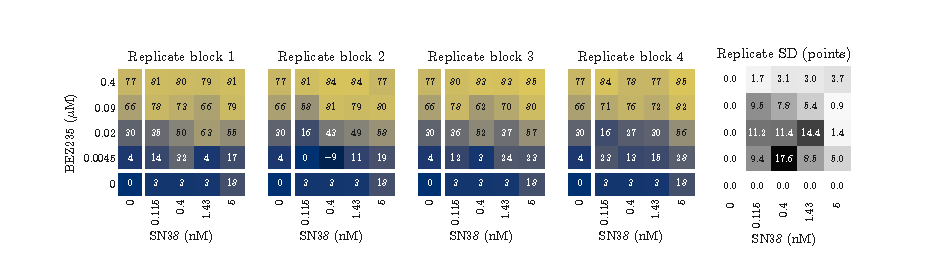
\includegraphics{figures/figS1_replicates.pdf}
\caption{\textbf{Single-agent values are shared by replicate blocks.} The four replicate blocks of the median pair-cell of main-text Figure 1 (BEZ235 + SN38 in DLD1). Single-agent edges (bottom row, left column) are identical in all four blocks; their standard deviation is zero (right), while the combination units vary between blocks. SN38 doses in nM, BEZ235 in µM.}\label{fig:S1}
\end{figure}

\paragraph{The second batch}

\begin{itemize}
\item The 1,260 blocks of the second batch have source rows of 2,273,700 or more.
\item In the 240 replicate pair-cells, the batch-2 single-agent edges equal the batch-1 values (largest difference 0.22, mean 0.002). The second batch therefore re-measured combinations, not single agents.
\item The other 75 re-measured pair-cells (5 pairs) changed the doses of one drug and are excluded from replicate analyses.
\end{itemize}
\paragraph{Frozen versus block-edge reference} The frozen Bliss reference (training-pair single-agent lookup) equals the block-edge reference everywhere except 604 units in 77 re-measured pair-cells. There the lookup mixes doses that differ between batches.

\section{Interaction targets}\label{sec:S2}
For unit $u$ in pair-cell $(p,c)$ let $\bar y_u$ be the replicate mean, $n_u$ the number of replicate rows and $E_u$ a reference. The pair-cell mean residual is $m_{pc}=w_{pc}^{-1}\sum_u n_u(\bar y_u-E_u)$ with $w_{pc}=\sum_u n_u$.

Within each panel $\mathcal P_{f,c}$ (the pairs of published fold $f$ in cell line $c$):

\begin{itemize}
\item let $H$ be the pair-by-drug indicator matrix, with $H_{pd}=1$ if drug $d$ belongs to pair $p$;
\item let $W=\operatorname{diag}(w_{\cdot c})$.
\end{itemize}
The \textbf{pair-cell contrast} is

\[
t_{\cdot c}=\{I-H(H^\top WH)^{+}H^\top W\}m_{\cdot c}.
\]
It is a $W$-orthogonal projection removing every additive drug-by-cell effect, including the cell mean, because the columns of $H$ sum to twice the constant vector. The \textbf{dose-shape contrast} applies the same construction to unit residuals after subtracting pair-cell means, with indicators of drug by dose rank.

Both are applied identically to targets, replicate half-differences and predictions. Energies are $\sum w t^2$. Four related targets are used:

\begin{itemize}
\item \textbf{measured-response contrast:} the same contrast of $\bar y_u$;
\item \textbf{reference-only contrast:} the contrast of $E_u$;
\item \textbf{HSA residual:} the contrast of $\bar y_u-\max(a_u,b_u)$;
\item \textbf{train-only target:} $m_{pc}$ minus an additive drug-by-cell baseline fitted only on pairs of other folds.
\end{itemize}
\section{Replicate noise}\label{sec:S3}
\setcounter{proposition}{3}
\begin{lemma}\label{lem:noise}
Assume:
\begin{itemize}
\item a panel has an even number $n$ of replicate blocks, $y_{ub}=\mu_u+\varepsilon_{ub}$;
\item block error vectors $\varepsilon_{\cdot b}$ are independent and identically distributed across blocks, with mean zero and arbitrary within-block covariance $\Sigma$;
\item the sign vector $\sigma\in\{\pm1\}^n$, with $n/2$ entries of each sign, is drawn independently of $\varepsilon$.
\end{itemize}
Let $d_u=n^{-1}\sum_b\sigma_by_{ub}$. Then $E\,d=0$ and $\operatorname{Cov}(d)=\Sigma/n=\operatorname{Cov}(\bar\varepsilon)$. Hence $E\|Cd\|_W^2=E\|C\bar\varepsilon\|_W^2$ for every fixed linear operator $C$ and weight $W$.
\end{lemma}
\begin{proof}
$\sum_b\sigma_b=0$ removes $\mu$. $\operatorname{Cov}(d_u,d_{u'})=n^{-2}\sum_b\sigma_b^2\Sigma_{uu'}=\Sigma_{uu'}/n$, which is the covariance of block means. Then $E\|Cd\|_W^2=\operatorname{tr}(C^\top WC\operatorname{Cov}d)$.
\end{proof}

Signs are assigned to whole blocks, so whole-block shifts count as noise. The lemma requires every unit to receive balanced signs. In 210 eight-block pair-cells the two sets of blocks have different dose labels: 135 differ by rounding and 75 genuinely. A split balanced over all eight blocks of a pair-cell then gives some units three signs of one kind and one of the other, which leaks dose-shape signal into $d$. Balancing within dose-grid groups restores the lemma. Table~\ref{tab:S2} compares the two splits; the per-pair-cell split overstates the dose-shape noise share.

The equivalent cross-product form is $t^2-d^2=t_At_B$ for the two half-sample targets, so the reproducible energy is the mean of $t_At_B$.

\begin{table}[H]
\centering
\small
\caption{\textbf{Noise shares (50 block-sign draws, seed 97).} The recomputation reproduces the frozen values bit for bit.}\label{tab:S2}
\begin{tabularx}{\linewidth}{@{}L r r r@{}}
\toprule
Estimate & Frozen & Recomputed & Batch-aware split \\
\midrule
Pair-cell Bliss noise share & 0.0978 [0.0893, 0.1077] & 0.0978 & 0.0971 \\
Pair-cell measured-response noise share & 0.0671 & 0.0671 &  \\
Dose-shape Bliss noise share, dose-grid split & 0.3633 [0.344, 0.382] & 0.3633 & 0.3631 \\
Dose-shape Bliss noise share, per-pair-cell split & 0.4473 & 0.4473 &  \\
\bottomrule
\end{tabularx}
\end{table}
\paragraph{Noise-corrected $R^2$} With $y$ the replicate-mean target, $e=y-\hat y$ the prediction error and $\hat N$ the estimated noise energy of $Cy$, this is $1-(\|Ce\|^2-\hat N)/(\|Cy\|^2-\hat N)$. It is a ratio of unbiased estimators, so it is consistent rather than unbiased. On the dose-shape Bliss contrast it is 0.240 for GP and 0.195 for the selected network; with the per-pair-cell split they are 0.278 and 0.226.

\section{Variance components and controls}\label{sec:S4}
The pair-wide component $\hat\tau^2$ is the row-weighted cross-cell U-statistic (main-text Eq. 5, Section 6.2), the weighted mean product of one pair's contrasts in two different cell lines. The pair-by-cell share is total minus noise minus pair-wide. The descriptive in-sample pair-mean share is reported separately because it includes noise and pair-by-cell variance divided by the number of cell lines.

\begin{table}[H]
\centering
\small
\caption{\textbf{Energy shares of the pair-cell contrast.} Pair-bootstrap intervals are shown for the main targets; for the Bliss target, drug and cell jackknife intervals are also given.}\label{tab:S3}
\begin{tabularx}{\linewidth}{@{}L r r r r@{}}
\toprule
Target & Noise & Pair-wide & Pair-by-cell & Descriptive pair mean \\
\midrule
Bliss residual & 0.098 & 0.242 [0.197, 0.293] & 0.660 [0.613, 0.702] & 0.254 \\
Bliss, drug jackknife & [0.070, 0.126] & [0.151, 0.334] & [0.566, 0.754] &  \\
Bliss, cell jackknife & [0.069, 0.127] & [0.160, 0.324] & [0.553, 0.767] &  \\
Measured response & 0.067 & 0.247 [0.214, 0.282] & 0.686 & 0.263 \\
Train-only baseline & 0.103 & 0.249 [0.195, 0.304] & 0.648 & 0.255 \\
HSA residual & 0.095 & 0.248 & 0.657 & 0.259 \\
Reference only & 0 & 0.264 & 0.736 & 0.286 \\
\bottomrule
\end{tabularx}
\end{table}
\paragraph{Reference contribution} Pair-wide covariance decomposes as $\tau^2_{raw}=\tau^2_{ref}+\tau^2_{bliss}+2\,\mathrm{cov}$: $7.41=2.44+4.99+2(-0.013)$. Pair means of the Bliss target correlate with:

\begin{itemize}
\item measured response, 0.81;
\item HSA, 0.98;
\item the train-only target, 0.80;
\item the reference alone, 0.009.
\end{itemize}
\begin{table}[H]
\centering
\small
\caption{\textbf{Controls (Bliss residual).}}\label{tab:S4}
\begin{tabularx}{\linewidth}{@{}L L@{}}
\toprule
Control & Result \\
\midrule
Pair labels permuted within (fold, cell) panels, 20 permutations & pair-wide 0.0007 ± 0.0016; leave-one-cell-out B1 $R^2$ −0.0001 \\
Zero interaction: reference plus block-sign-flipped replicate deviations, 5 realizations & noise share 0.988 (0.974–1.004); pair-wide −0.0009; B1 0.000; B2 −0.001 \\
Single-agent values perturbed with SD 2 / 5 / 10 points & 0.25\% / 1.6\% / 6.4\% of target energy; pair-wide share 0.246 / 0.243 / 0.234 \\
\bottomrule
\end{tabularx}
\end{table}
The noise-corrected 39 × 39 cross-cell covariance has a leading eigenvalue holding 30.6\% of its trace; that eigenvector has cosine 0.94 with the constant vector. The next four eigenvalues hold 13.9\%, 9.8\%, 8.0\% and 6.7\%.

\section{Same-pair information experiments}\label{sec:S5}
\paragraph{Design} The design was committed before outcomes were computed (\file{experiments/interaction_gap_20261110/design.json}).

\begin{itemize}
\item \textbf{Anchor masks.} For each held-out pair and seed (20 seeds), cell lines are permuted using a SHA-256 hash of (pair, seed). Anchors are the first $k$; evaluation uses positions 16–38 for every $k$ and model.
\item \textbf{B1} uses $\hat\tau^2$ and $\hat s^2$ from the four non-test folds.
\item \textbf{B2} uses the signal covariance $K=\lambda K_{CS}+(1-\lambda)(U_r\Lambda_rU_r^\top+\Psi)$ with $\lambda\in\{0,0.25,0.5,0.75,1\}$ and $r\in\{1,2,3,5,8,12,20,38\}$. These are chosen per (target, fold, $k$) on validation fold $f+1$, with covariance from the other three folds, then refitted.
\item \textbf{Controls.} B4 feeds B1 or B2 the anchors of a training-fold donor pair that shares exactly one drug with the evaluated pair, and B5a those of a donor pair that shares none. B5b feeds B2 the pair's own anchor contrasts with their cell lines deranged. B0 predicts zero.
\item \textbf{Leakage test.} Setting the targets of the evaluated cell lines to +100 leaves the B1 and B2 predictions unchanged.
\end{itemize}
\begin{table}[H]
\centering
\small
\caption{\textbf{Anchor curve on the Bliss contrast.} The 23 evaluation cell lines are identical for every $k$; values are pooled $R^2$ with pair-bootstrap intervals.}\label{tab:S5}
\begin{tabular*}{\linewidth}{@{\extracolsep{\fill}}r r r r r r r@{}}
\toprule
$k$ & B1 & B2 & B2 − B1 & Donor sharing a drug (B2) & Unrelated donor (B2) & Deranged (B2) \\
\midrule
1 & 0.049 & 0.081 & 0.033 [0.024, 0.041] & −0.087 & −0.091 & — \\
2 & 0.083 & 0.130 & 0.047 [0.038, 0.056] & −0.132 & −0.136 & −0.013 \\
4 & 0.123 & 0.178 & 0.055 [0.047, 0.063] & −0.176 & −0.193 & 0.040 \\
8 & 0.164 & 0.227 & 0.063 [0.054, 0.072] & −0.213 & −0.231 & 0.089 \\
16 & 0.194 & 0.280 & 0.086 [0.071, 0.102] & −0.267 & −0.286 & 0.085 \\
\bottomrule
\end{tabular*}
\end{table}
At $k=16$:

\begin{itemize}
\item \textbf{Targets.}
\begin{itemize}
\item Train-only target: B1 0.196, B2 0.283.
\item Measured response: B1 0.204, B2 0.317.
\item Bliss minus the held-out-pair F2 prediction: B1 0.226, B2 0.288.
\item Reference only: B1 0.229, B2 0.476.
\end{itemize}
\item \textbf{Residual after the offset.} B2 removes 10.7\% [8.9, 12.6] of the energy left after B1, which is 12.2\% of the reproducible part of that residual.
\item \textbf{Error scale.} RMSE is B0 4.54, B1 4.08, B2 3.85.
\item \textbf{Across seeds and folds.} The SD of pooled $R^2$ across anchor seeds is 0.006 (B1) and 0.009 (B2). B2 exceeds B1 in all five folds.
\end{itemize}
\paragraph{Matched comparison} The pair-cell split assigns each pair's cell lines round-robin to five folds. With test fold $f$ and validation fold $f+1$, anchors are the pair's cell lines in the other three folds.

The frozen contrast fits drug effects within panels that mix training and test entries. Anchors built from it therefore carry other pairs' test entries, and a covariance estimated on training entries of those panels picks up test entries through the drug fit.

\begin{table}[H]
\centering
\small
\caption{\textbf{Matched B1 and B2 under the frozen and the leak-free contrast (fixed $\lambda=0.5$, full rank).}}\label{tab:S6}
\begin{tabularx}{0.6\linewidth}{@{}L r r@{}}
\toprule
Anchors / covariance & B1 & B2 \\
\midrule
frozen / frozen & 0.209 & 0.308 \\
frozen / leak-free & 0.208 & 0.262 \\
leak-free / frozen & 0.183 & 0.256 \\
leak-free / leak-free & 0.177 & 0.209 \\
\bottomrule
\end{tabularx}
\end{table}
With selected settings, the leak-free B2 is 0.216.

\begin{figure}[H]
\centering
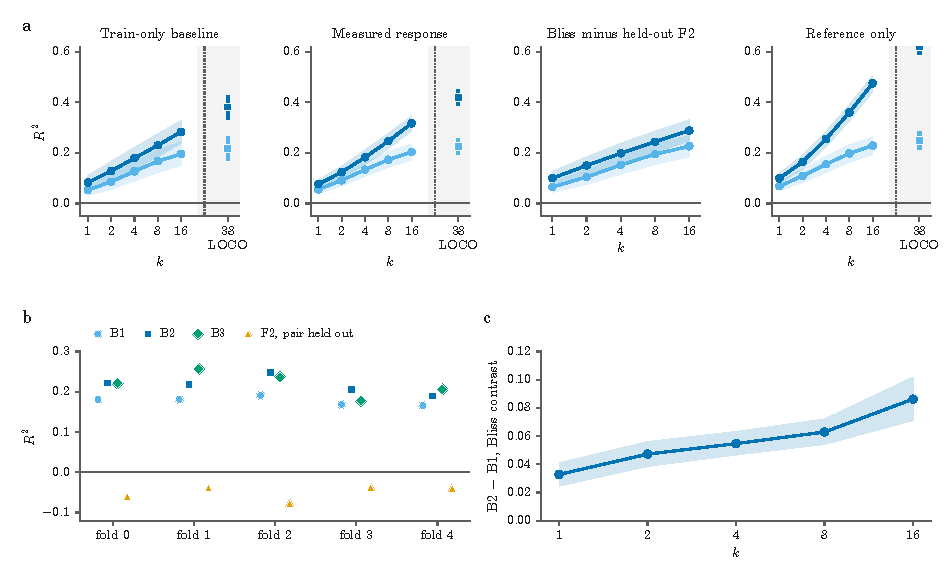
\includegraphics{figures/figS2_anchor_robustness.pdf}
\caption{\textbf{Same-pair transfer for other targets and by fold.} \textbf{(a)}~Anchor curves as in main-text Figure 5a for four other targets: the Bliss residual with a drug-by-cell baseline fitted only on other folds (train-only), the measured-response contrast, the Bliss residual minus the held-out-pair F2 prediction, and the reference-only contrast. Light blue, B1; dark blue, B2; bands, 95\% pair-bootstrap intervals; squares, each cell line predicted from the pair's 38 others where computed. \textbf{(b)}~Leak-free matched comparison by pair-cell-split fold (Table~\ref{tab:S7}). \textbf{(c)}~B2 − B1 on the Bliss contrast against the number of anchors $k$, with 95\% pair-bootstrap intervals (Table~\ref{tab:S5}).}\label{fig:S2}
\end{figure}

\begin{table}[H]
\centering
\small
\caption{\textbf{Leak-free matched comparison by pair-cell-split fold.} B3 values were recomputed from the 15 saved prediction files; the pooled B3 $R^2$ 0.2182355 equals the campaign record exactly.}\label{tab:S7}
\begin{tabularx}{0.75\linewidth}{@{}L r r r r r@{}}
\toprule
Fold & 0 & 1 & 2 & 3 & 4 \\
\midrule
B1 & 0.181 & 0.181 & 0.190 & 0.168 & 0.166 \\
B2 & 0.222 & 0.218 & 0.247 & 0.206 & 0.189 \\
B3 & 0.221 & 0.256 & 0.236 & 0.178 & 0.206 \\
Held-out-pair F2 & −0.060 & −0.039 & −0.077 & −0.037 & −0.040 \\
\bottomrule
\end{tabularx}
\end{table}

\section{Cross-batch reproducibility}\label{sec:S6}
For the 240 replicate pair-cells, each batch alone (weight 64) replaces the pair-cell mean in the frozen contrast; noise is estimated within batch. With $t_1$, $t_2$ the batch targets and $v_b$ the within-batch noise, the moments are:

\begin{itemize}
\item within-batch reproducible energy $E[t_b^2]-v_b$;
\item cross-batch energy $E[t_1t_2]$;
\item within-batch cross-cell products $E[t_{b,c}t_{b,c'}]$;
\item cross-batch cross-cell products $E[t_{1,c}t_{2,c'}]$.
\end{itemize}
Intervals are a 2,000-draw bootstrap over the 16 pairs.

\begin{table}[H]
\centering
\small
\caption{\textbf{Moments of the Bliss contrast (contrast units squared).}}\label{tab:S8}
\begin{tabularx}{0.85\linewidth}{@{}L r r@{}}
\toprule
Quantity & Unadjusted & Cell-line batch shift removed \\
\midrule
Within-batch reproducible & 38.5 & 41.0 \\
Cross-batch & 18.3 & 36.0 \\
Ratio, overall & 0.48 [0.08, 0.74] & 0.88 [0.65, 1.01] \\
Ratio, pair-wide & 0.27 & 0.89 [0.52, 0.97] \\
Ratio, pair-by-cell & 0.68 & 0.85 [0.62, 1.16] \\
Mean squared difference / within-batch noise & 4.47 & 1.79 \\
\bottomrule
\end{tabularx}
\end{table}
Removing the shift is appropriate because a complete re-run would absorb a cell-line shift through the contrast. The measured-response contrast gives a ratio of 0.89. Using each batch's own single-agent edges changes nothing, because they are the same values.

\paragraph{Extrapolation} Batch-specific energy is 5.0 squared units against a within-batch noise of 5.7 per batch. If batch variance scales with replicate noise, the full-screen batch share is about 0.08 and the cross-batch reproducible share about 0.82. If batch variance is constant in absolute terms, the batch share is about 0.23 and the reproducible share about 0.67.

The re-tested pairs have pair-wide share 0.449 and energy 26.9 per row against 0.242 and 20.6 for all pairs, so neither assumption can be checked here.

\paragraph{Transfer to the other batch} Leave-one-cell-out B1 and B2 from batch-1 anchors give the following $R^2$:

\begin{itemize}
\item against batch 1: B1 0.464, B2 0.497 (gain 0.033 [−0.030, 0.106]);
\item against batch 2: B1 0.492, B2 0.523 (gain 0.030 [−0.015, 0.086]).
\end{itemize}

\begin{figure}[H]
\centering
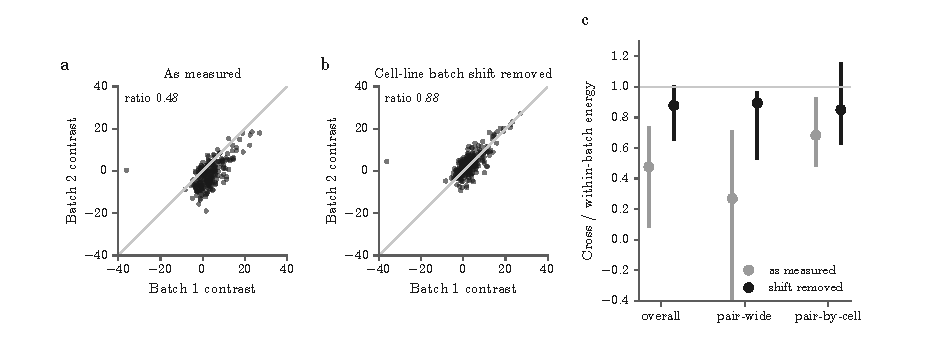
\includegraphics{figures/figS3_cross_batch.pdf}
\caption{\textbf{Cross-batch replication.} The 240 pair-cells (16 pairs) measured in two batches with the same doses. \textbf{(a)}~Bliss contrasts of each batch alone, as measured. \textbf{(b)}~After removing a cell-line batch shift. \textbf{(c)}~Ratio of cross-batch to within-batch reproducible energy, overall and by component, with 95\% bootstrap intervals over the 16 pairs (Table~\ref{tab:S8}); grey, as measured; black, shift removed.}\label{fig:S3}
\end{figure}

\section{Grounding of the cross-cell structure}\label{sec:S7}
Cell-line similarity was taken from DeepSynergy expression features (FARMS-summarized, 3,984 genes), which are independent of combination outcomes \citep{preuer2018}.

\begin{itemize}
\item \textbf{Stability.} The noise-corrected correlation of pair-centred contrasts across cell lines is reproducible across disjoint halves of the pairs (Spearman 0.62, $p=0.0005$; measured response 0.72).
\item \textbf{Mantel test against expression similarity.} Bliss: $\rho=0.069$, $p=0.082$. Measured response: 0.121, $p=0.002$. 10,000 permutations each.
\item \textbf{Expression-only predictor.} A leave-one-cell-out predictor whose cell similarity comes from expression gains 0.002 [−0.002, 0.006] over B1, 1.1\% of B2's gain.
\end{itemize}
\section{Zero-interaction control}\label{sec:S8}
The zero-interaction protocol (scripts r16–r21) was frozen in October 2026 and re-executed for this paper. All committed numeric outputs and tables reproduced with maximum absolute difference 0.

\paragraph{Construction}
\begin{itemize}
\item \textbf{Simulated screen.} Responses are a non-interaction reference plus noise, with no true interaction. Each block is then scored by the native Loewe pipeline and by Bliss.
\item \textbf{Learners.} Neighbourhood CF and pair-kernel ridge regression are trained on held-out pairs to predict the contrast of each label.
\end{itemize}
\begin{table}[H]
\centering
\small
\caption{\textbf{The zero-parameter term $M=R_{\mathrm{Bliss}}-R_{\mathrm{Loewe}}$ and its parts} (contrast $R^2$ against the observed Loewe label; parts as defined in main-text Figure 6d), with the role of the fallback.}\label{tab:S9}
\begin{tabularx}{0.7\linewidth}{@{}L r@{}}
\toprule
Component & Value \\
\midrule
Zero-parameter single-agent term $M$ & 0.772 \\
Implementation part $M_{impl}$ & 0.752 \\
Existence part $M_{exist}$ & 0.703 \\
Algebraic part $M_{alg}$ & −0.047 \\
Share of units involving the fallback & 0.798 \\
Share of $M_{impl}$ energy in fallback units & 0.917 \\
\bottomrule
\end{tabularx}
\end{table}
A network using single-agent inputs only predicts the held-out Loewe contrast with $R^2$ 0.307 but the Bliss contrast with 0.003.

\paragraph{Limitations}
\begin{itemize}
\item The simulation fixes one reference and one noise model.
\item It shows that Loewe labels can carry learnable reference structure. It does not show that observed screens lack interaction, nor that Loewe values are erroneous.
\end{itemize}
\paragraph{Reference cancellation} If $\hat S=\hat Y-R$ and $S=Y-R$ for a reference $R$ fixed before outcomes, then $\hat S-S=\hat Y-Y$. A model trained on responses therefore has the same error on any such score as on the response.

\section{Proofs for the Loewe reference}\label{sec:S9}
Propositions 1--3 are stated in main-text Section 8.2; Proposition 5 is stated here.
\paragraph{Setting} An arm is $f(x)=c+(d-c)/\{1+(x/e)^b\}$, $x>0$, with $e>0$, $b\neq0$, $c\neq d$. It is increasing if and only if $(b<0,d>c)$ or $(b>0,d<c)$. Its plateaus are $\ell_f=\lim_{x\to0^+}f$ and $h_f=\lim_{x\to\infty}f$.

On the open interval between $c$ and $d$ the inverse is $D(y)=e\{(d-y)/(y-c)\}^{1/b}$, continuous and strictly increasing for an increasing arm. For co-increasing arms of drugs 1 and 2 at positive doses $x_1,x_2$, with common interval $(\ell,h)=(\max_k\ell_k,\min_kh_k)\neq\emptyset$, let $g(y)=x_1/D_1(y)+x_2/D_2(y)-1$, and label the arms $i,j$ so that $h_i\le h_j$.

\begin{proof}[Proof of Proposition 1]
\begin{enumerate}
\item Each $D_k$ is continuous and strictly increasing on a range containing $(\ell,h)$. So each $x_k/D_k$ is strictly decreasing, and so is $g$.
\item As $y\to\ell^+$, an arm with $\ell_k=\ell$ has $D_k\to0^+$, so its term diverges because $x_k>0$; the other term is positive.
\item As $y\to h_i^-$, $D_i\to\infty$. Because $h_i$ lies inside arm $j$'s range when $h_i<h_j$, $D_j(h_i)$ is finite and positive, so $g\to x_j/D_j(h_i)-1$.
\item That limit is negative if and only if $x_j<D_j(h_i)$, if and only if $f_j(x_j)<h_i$, since $f_j$ is strictly increasing with $f_j(D_j(h_i))=h_i$.
\item If $h_i=h_j$, both inverses diverge and the limit is $-1$.
\item Continuity, strict monotonicity and the intermediate value theorem give existence and uniqueness.\qedhere
\end{enumerate}
\end{proof}
Co-decreasing arms reduce to this case under $y\mapsto-y$. Arms of opposite monotonicity, flat arms and empty common intervals are outside the statement.

\begin{proof}[Proof of Proposition 2]
\begin{enumerate}
\item Let doses converge to $(\bar x_i,\bar x_j)\in B$, so $\bar x_j=D_j(h_i)$. For fixed $\varepsilon>0$, $g(h_i-\varepsilon)\to\bar x_i/D_i(h_i-\varepsilon)+D_j(h_i)/D_j(h_i-\varepsilon)-1$. The second ratio exceeds 1, so the limit is positive. For nearby doses $g(h_i-\varepsilon)>0$, and monotonicity gives $y^*\in(h_i-\varepsilon,h_i)$. Since $\varepsilon$ is arbitrary, $y^*\to h_i$.
\item On the no-root side $f_j(x_j)\ge h_i>f_i(x_i)$, so HSA equals $f_j(x_j)$, which is the continuous extension.
\item On $B$, $x_1+x_2>x_j$ because $x_i>0$, and $f_j$ is strictly increasing, so $\max_kf_k(x_1+x_2)>f_j(x_j)=h_i$. With $h_i<100$ this gives $J>0$.\qedhere
\end{enumerate}
\end{proof}
Off the boundary, $J$ evaluated at the actual doses can be close to zero: if the stronger arm is already near its plateau, $f_j(x_1+x_2)\approx f_j(x_j)$. This is why only 58\% of rejected roots near a weaker-drug plateau below 100 show a positive jump. For those roots the identity native − certified $=J+(h_i-y^*)$ was checked to $3\times10^{-12}$.

\begin{proof}[Proof of Proposition 3]
\begin{enumerate}
\item The root equation $x_i/D_i(y^*)=\delta(y^*)$, with $\delta(y)=1-x_j/D_j(y)$, gives $(h_i-y^*)/(y^*-\ell_i)=\tilde q=\{\delta(y^*)e_i/x_i\}^{|b_i|}$ under either sign convention of $b_i$. Hence $h_i-y^*=|d_i-c_i|\,\tilde q/(1+\tilde q)$ exactly.
\item The function $\delta(y)$ is increasing, so $\delta(y^*)<\delta=\delta(h_i)$ and, by step 1, $h_i-y^*\le|d_i-c_i|\,q$ with $q=(\delta e_i/x_i)^{|b_i|}$; hence $h_i-y^*=O(\delta^{|b_i|})$. Since $h_i<h_j$, $D_j$ is $C^1$ near $h_i$, so $|\delta(y^*)-\delta|=O(h_i-y^*)=O(\delta^{|b_i|})$.
\item Then $\tilde q/q=\{\delta(y^*)/\delta\}^{|b_i|}=1+O(\delta^{|b_i|-1})\to1$ for $|b_i|>1$. Since also $q\to0$, step 1 gives $h_i-y^*=|d_i-c_i|\,\tilde q/(1+\tilde q)\sim|d_i-c_i|\,q$.\qedhere
\end{enumerate}
\end{proof}
\setcounter{proposition}{4}
\begin{proposition}[replicates sharing a reference cannot rank conventions]\label{prop:replicates}
Let block scores be $S^v_{ub}=y_{ub}-R^v_u$, where every convention's reference depends only on inputs shared by the blocks of unit $u$. Then:

\begin{itemize}
\item $S^v_{ub}-S^v_{ub'}=y_{ub}-y_{ub'}$, so any statistic that depends on a unit's block scores only through their differences (within-unit variances, ranges, sign-split contrasts) takes the same value under all conventions; unit means and other statistics that are not shift-invariant change with $R^v_u$;
\item the intraclass reliability of unit means over $m$ blocks is $\rho_v=V_v/(V_v+\sigma^2/m)$ with $V_v=\operatorname{Var}_u(\mu_u-R^v_u)$, so adding to $R^v$ any non-constant deterministic artifact uncorrelated with $\mu-R^v$ increases $V_v$ and therefore $\rho_v$.
\end{itemize}
\end{proposition}
Replicate agreement therefore cannot select a convention when single-agent values are shared.

\paragraph{Unresolved: solver rejection} The mechanism of native Newton rejection is a conjecture: iterates leave $(\ell,h_i)$ when the boundary layer is thinner than the first step. It is supported by the slope concentration and by a start-point intervention (102 of 400 acceptance changes, 68 with certified roots), but is not proved.

\section{Numerical certification and counts}\label{sec:S10}
\begin{table}[H]
\centering
\small
\caption{\textbf{Native solver codes on all 367,152 cases.}}\label{tab:S10}
\begin{tabularx}{0.5\linewidth}{@{}L r@{}}
\toprule
Native code & Cases \\
\midrule
1 & 182,162 \\
2 & 85 \\
3 & 137,642 \\
6 & 8 \\
999 (no attempt or error) & 47,255 \\
\bottomrule
\end{tabularx}
\end{table}
Native accepted 182,247 cases and fell back on 184,905.

The populations of main-text Table 4 are disjoint, and their certificate classes sum to 367,152:

\begin{itemize}
\item certified root 195,984 (180,364 accepted + 15,620 rejected);
\item certified no root 117,824;
\item undefined opposite or flat 49,184;
\item empty interval 4,160.
\end{itemize}

\paragraph{Certificates} Each case was evaluated in 100-digit interval arithmetic (mpmath), with the stored float64 fit coefficients taken as exact binary rationals. Because $g$ is strictly monotone on $(\ell,h)$, with one end diverging and the other having a finite limit $g_{\mathrm{end}}$, a root exists if and only if $g_{\mathrm{end}}$ has the opposite sign to the diverging end. A case is a certified root when a bracket $[y_0,y_1]$ strictly inside $(\ell,h)$ has interval enclosures of $g(y_0)$ and $g(y_1)$ of strictly opposite signs, and a certified no-root case when the enclosure of $g_{\mathrm{end}}$ lies strictly on the same side of zero as the diverging end. Cases whose enclosure of $g_{\mathrm{end}}$ contains zero are left unresolved; no case of this screen is.

\paragraph{C1 and C2} C1 roots are confirmed in double precision by two independent checks: the root satisfies the native Loewe equation and lies strictly inside both fitted effect ranges, and a second root finder that never inverts a curve (bisection on the dose fraction $x_1/D_1(y)$) finds it. C1 (14,197) contains:

\begin{itemize}
\item 12,477 cases where the solver stopped at the root but the answer was discarded;
\item 1,720 cases where the root exists but the solver failed.
\end{itemize}
C2 (1,423) contains boundary roots within about $10^{-13}$ of a plateau, where float64 residuals cannot separate root from asymptote and only the 100-digit certificate does. $\mathrm{C1}\cup\mathrm{C2}$ equals the 15,620 rejected certified roots exactly.

\begin{figure}[H]
\centering
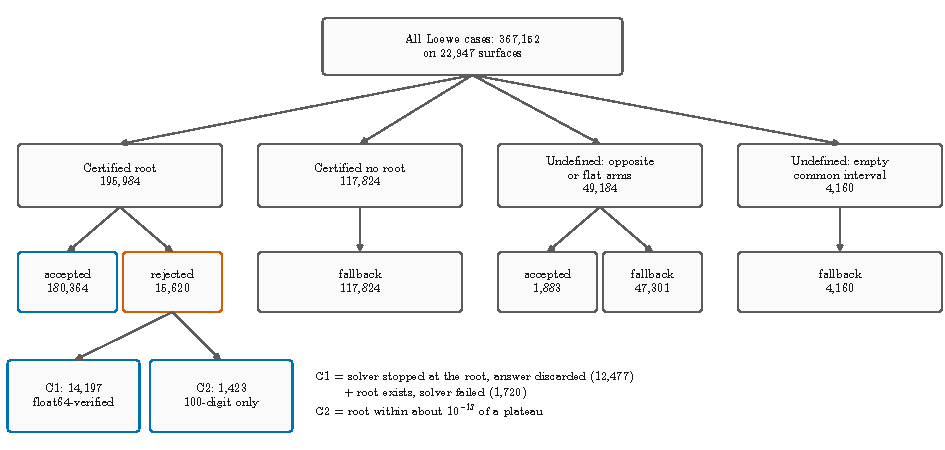
\includegraphics{figures/figS4_loewe_populations.pdf}
\caption{\textbf{Nesting of the Loewe case populations.} All 367,152 cases by certificate status, native solver outcome and, for rejected certified roots, the C1/C2 split (main-text Table 4). Counts are disjoint within a level and nest across levels.}\label{fig:S4}
\end{figure}

\paragraph{Checks}

\begin{itemize}
\item \textbf{Existence criterion.} Against certificates it agrees in all 310,928 co-monotone LL.4 cases, with 0 near-ties needing 60-digit arithmetic; 4,576 cases with an L.4 arm are excluded.
\item \textbf{Bracket replay.}
\begin{itemize}
\item Rejected roots: 15,588/15,588 confirmed.
\item Accepted controls: 1,994/1,994.
\item Accepted roots near an asymptote: 2,443/2,443.
\end{itemize}
\end{itemize}
\section{Fallback errors and jump}\label{sec:S11}
\begin{table}[H]
\centering
\small
\caption{\textbf{Absolute error of each fallback against the certified root (inhibition points).}}\label{tab:S11}
\begin{tabularx}{\linewidth}{@{}L l r r r@{}}
\toprule
Population & Fallback & Median & Mean & 90th percentile \\
\midrule
C1, 14,197 & Summed dose & 4.17 & 20.85 & 70.9 \\
C1, 14,197 & HSA & 0.0040 & 0.72 & 1.28 \\
C2, 1,423 & Summed dose & 4.02 & 21.54 & 71.1 \\
C2, 1,423 & HSA & 0.0000 & 0.29 & 0.33 \\
\bottomrule
\end{tabularx}
\end{table}
HSA is closer in 71.7\% of C1 cases.

\paragraph{Where the C1 roots lie} Of the 13,856 co-increasing LL.4 C1 roots:

\begin{itemize}
\item 10,712 lie within 0.01 of the upper plateau and carry 68.3\% of the absolute reference shift; 10,646 of these have a plateau below 100;
\item 1,608 lie near the lower asymptote (20.4\%);
\item 1,536 are interior (11.3\%).
\end{itemize}
For the 10,646, the jump $J$ has median 3.83 and mean 18.9 and is positive in 58\%.

\paragraph{Boundary layer} For 13,277 certified roots within 0.01 of the smaller plateau:

\begin{itemize}
\item the median absolute $\log_{10}$ ratio of predicted to certified distance is $2.7\times10^{-5}$;
\item 94.0\% fall within 1\% and 97.7\% within a factor of 2;
\item the log–log correlation is 0.998.
\end{itemize}

\begin{figure}[H]
\centering
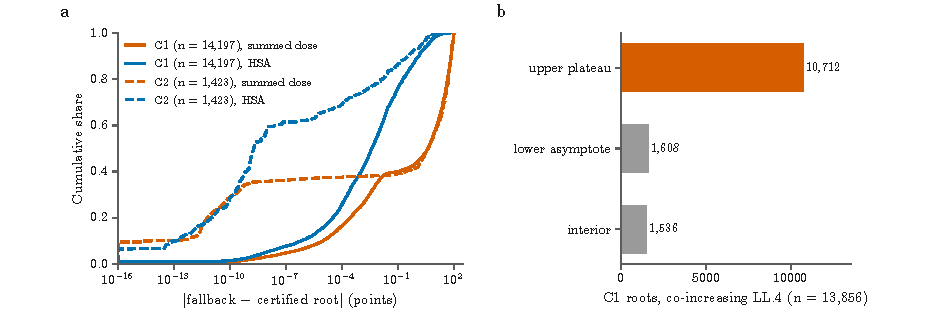
\includegraphics{figures/figS5_fallback_errors.pdf}
\caption{\textbf{Fallback error by population and location of rejected roots.} \textbf{(a)}~Cumulative distribution of the absolute difference between each fallback and the certified root for C1 and C2 (Table~\ref{tab:S11}); differences below $10^{-16}$ are drawn at $10^{-16}$. \textbf{(b)}~Location of the 13,856 co-increasing LL.4 C1 roots: within 0.01 of the upper plateau, near the lower asymptote, or interior.}\label{fig:S5}
\end{figure}

\section{Screening analysis}\label{sec:S12}
\paragraph{Fidelity} Native block scores reproduce the stored reconstruction exactly. Against published DrugComb scores they have:

\begin{itemize}
\item RMSE 0.704 and correlation 0.9990;
\item 92.3\% of scores within 0.01;
\item top-5\% list differing by 1 of 1,137.
\end{itemize}
\begin{table}[H]
\centering
\small
\caption{\textbf{Turnover of the top list by budget (native to C1).} No budget has ties at its cutoff.}\label{tab:S12}
\begin{tabularx}{0.6\linewidth}{@{}L r r r@{}}
\toprule
Budget & Selected & Replaced & Turnover \\
\midrule
1\% & 228 & 19 & 8.33\% \\
2\% & 455 & 33 & 7.25\% \\
5\% & 1,137 & 67 & 5.89\% \\
10\% & 2,274 &  & 5.72\% \\
20\% & 4,548 &  & 5.23\% \\
\bottomrule
\end{tabularx}
\end{table}
At the 5\% budget, other changes give different turnovers:

\begin{itemize}
\item restoring all 15,620 roots (I): 6.95\%;
\item HSA fallback for all no-root cases (H): 30.87\%;
\item both (IH): 30.78\%;
\item from I to IH: 26.74\%.
\end{itemize}
\paragraph{Entrants and exits} Entrants sat a median 3.60 below the native cutoff (90th percentile 11.07, maximum 25.87; 10 within one point). Their scores rose by a median 6.06 and a mean 8.11. Exits sat a median 0.167 above the cutoff, and their scores did not change (maximum absolute change 0.023).

C1 changes 5,003 pair-cell scores and reverses 517 pair-cell signs.

\paragraph{Resampling} The resampling analysis uses 1,000 bootstrap resamples and 200 half-depth splits of combination replicates.

\begin{itemize}
\item The native-to-C1 turnover is 5.87\% [5.10, 6.68] (bootstrap) and 5.77\% (half-depth).
\item Replicate noise alone turns over 16.6\% (consecutive bootstrap draws) and 28.5\% (half-depth).
\end{itemize}
\section{Negative and inconclusive results}\label{sec:S13}
\begin{table}[H]
\centering
\small
\caption{\textbf{Hypotheses that were not supported, with sources (under \texttt{results/} unless stated).}}\label{tab:S13}
\begin{tabularx}{\linewidth}{@{}L L L@{}}
\toprule
Hypothesis & Result & Source \\
\midrule
NCATS confirmation of high-inhibition specificity & H1: $R^2$ 0.057 (seeds 0.065, 0.042, 0.064), drug jackknife [−0.006, 0.120], rule not met; sequence stopped & \file{mechanisms_20261108/historical_controls/failed_ncats_confirmation.json} \\
Drug identity costs at least 5\% response MSE & +4.61\% pooled over seeds 2026–2029 (Holm $p$ 0.0048), below threshold; seed 2029 +3.23\% & \file{final_20261110/claim_ledger.json} (I1) \\
Removing drug identity improves the contrast & −7.41\% [drug −15.3, 0.5]; Bliss-residual objective −3.85\% & \file{reports/final_20261110/FINAL_RESEARCH_VERDICT.md} \\
Identity channels interact & +2.21\%, Holm $p$ 0.38 & \file{mechanisms_20261108/gpu_return/joint_identity/comparisons.csv} \\
Uncertainty utility & Frozen rule unmet (GP and network ensembles) & \file{reports/final_20261110/FINAL_RESEARCH_VERDICT.md} \\
Dose-aware DeepSynergy adaptation & Shared response task: RMSE 18.19, $R^2$ 0.713, measured-response contrast $R^2$ 0.283 & \file{compare/final.csv} \\
\bottomrule
\end{tabularx}
\end{table}
\section{Reproducibility}\label{sec:S14}
{\raggedright
All commands run from the repository root at the manuscript commit, with Python 3.14, numpy 2.4.1, pandas 2.3.3, scipy 1.17.0, matplotlib 3.10.8 and mpmath. The native Loewe references were computed with the SynergyFinder 2.0.12 Loewe code under R 3.6.3 and nleqslv 3.3.2. Table~\ref{tab:S14} gives the SHA-256 of every input and Table~\ref{tab:S15} those of the saved pair-seen predictions. The commands refer to these directories:
\begin{itemize}
\item \texttt{RES}: \file{results/research_20261107/resolution} on branch \texttt{research/resolution-reliability} (d2c8f41), the frozen out-of-fold unit means;
\item \texttt{RES\_B2}: the columns of \texttt{RES} holding the truth, the production F2 seeds and the Bliss reference, copied exactly;
\item \texttt{NATIVE}: \file{results/neural/runs/scientific_native_full}, the native SynergyFinder run;
\item \texttt{LOEWE}: the Loewe certificates, float64-verified cases and case regimes of Table~\ref{tab:S14};
\item \texttt{RUNS}: \file{results/final_20261110/runs} in the cluster run clone at 8bce416, holding the 15 prediction files;
\item \texttt{GAP\_DERIVED}, \texttt{AUDIT\_DERIVED}: directories outside the repository for per-pair-cell and per-case tables, which are regenerated rather than redistributed;
\item \texttt{GATE2}, \texttt{COMMITTED}: two checkouts of \texttt{main} at ae55c68; the zero-interaction (Gate 2) pipeline frozen in October 2026 is re-executed in the first and compared with the committed outputs of the second.
\end{itemize}
\par}

\begin{table}[H]
\centering\footnotesize
\caption{\textbf{SHA-256 of every input.} Raw files are verified by \texttt{cs622.download}; the split is hashed with LF line endings, as committed.}\label{tab:S14}
\begin{tabularx}{\linewidth}{@{}>{\raggedright\arraybackslash}X >{\ttfamily\scriptsize}l@{}}
\toprule
Input & \normalfont\footnotesize SHA-256 \\
\midrule
DrugComb v1.4 dose-response table, \file{data/raw/drugcomb/drugcomb_data_v1.4.csv} & 58c3893c9b8973eaea22aee819c0f268b3739d091a1d451187c1488c1058fe1d \\
DrugComb v1.4 summary table, \file{data/raw/drugcomb/summary_table_v1.4.csv} & e08e3d35bfa4bea011afe1b05b7025acde5c669c5e8d265866b5e12b08037a2f \\
DeepSynergy labels, \file{data/raw/deepsynergy/labels.csv} & 4ef40678fff51faa84fa4de63344c5b51e2e4abe7c28a417af24ec2b50fa135a \\
DeepSynergy feature archive, \file{data/raw/deepsynergy_original/X.p.gz} & e399f6cdb40184048ac34b370f89cc6e4582bec72893cc2c98d90c1634517899 \\
\addlinespace
O'Neil observation table, \file{data/processed/oneil_v1/observations.parquet} & ea588405019971906ac99c3caa547d5f4fac5b1be340356f0a8fe17a6aa3ce8b \\
Expression features, \file{data/processed/deepsynergy/features.npz} & 4ece7882cbc3e1576bc7400d5c2f53d48d466de9eaafbc5d69ff1bb547d7f40d \\
Pair-cell split, \file{results/final_20261110/oracle/pair_cell_split.csv} & d32914a94d8ead90e12d8cb10b6beed15f93339b0de2200ce2075a67a79370ea \\
\addlinespace
\texttt{RES}/\file{cache.npz} & 91f93811dedf5c0721198146638c21f25b1616d43f43ae9322cf8790a7e86687 \\
\texttt{RES}/\file{coordinates.parquet} & ebdcf3090da9bf8bf9aede5281990b843df4befc02e429bc9972a886044896d1 \\
\texttt{RES}/\file{inputs.json} & 8b81e6e3f526e232f0269c826ad26dcbe8f0466297521e2cf60b68696afc78f4 \\
\texttt{RES}/\file{variance.json} & 4393fa99455217fe29709a0761fa0c4a5fbf42cbf9226fdc529110cc37f3284c \\
\texttt{RES}/\file{error_decomposition.csv} & f475aab09e8849a305f7302f3ff237384ef160e1137558aaf8e8fdf99ad76e7e \\
\texttt{RES\_B2}/\file{cache.npz} & 8d3cb446659d8cb120b813d0f5f12f95e0abaaf4ccfd0d9ed7cc0b41b448dee4 \\
\addlinespace
\texttt{NATIVE}/\file{blocks.parquet} & 866ae92c09829e25dde86e139a83d6a9be11fe335b024b530141243d7f13f169 \\
\texttt{NATIVE}/\file{panel.parquet} & cc314c726f7e161dab0d49cc2edc49606805b1a2945889bdf68e0f527456a9bc \\
\texttt{NATIVE}/\file{surface_cases.parquet} & 69e2c76476c8d14aa3c289b0a98ad6703b40b7eb9ad903f9e2df2cd1d4e23528 \\
\texttt{LOEWE}/\file{certificates_replayable.parquet} (\texttt{cs622.certificate\_audit}) & 7087e8531dfdf595e81a6b745861459cdc37c1b2bb110da2f7e2cb41381c9728 \\
\texttt{LOEWE}/\file{cases_verified.parquet} (\texttt{cs622.loewe\_verify}) & 384a2bd51b4c9ffeca7d4d1768237a6212bf5cf126b2c16a382af87d72acf438 \\
\texttt{LOEWE}/\file{loewe_regimes.csv} (\file{experiments/overnight_20261107/regimes_and_tests.py}) & 9129a93bb77634db885bf8c7854c3314e9cd8ef4c377d98e74011fd2bff1fbc7 \\
\addlinespace
\texttt{GATE2}/\file{results/preliminary/r18_gate2.json} & 9db2939781ded864e55401b1a28523a588b3ff0502c794f37a7e5464e8616aa4 \\
\texttt{GATE2}/\file{results/preliminary/r18_units.npz} & d55477283e0fadd3a9e983586d36e3f12731a7b0a5132c09f6a1da6ad956367e \\
\bottomrule
\end{tabularx}
\end{table}

\begin{table}[H]
\centering\footnotesize
\caption{\textbf{SHA-256 of the 15 pair-seen prediction files} \texttt{RUNS/f2\_pair\_seen/seed\_}\textit{s}\texttt{/fold\_}\textit{f}\texttt{/predictions.parquet}, as recorded by the pair-seen audit (\texttt{pairseen\_audit.json}); all 15 matched again before the paired B3 comparison.}\label{tab:S15}
\begin{tabular}{@{}l l >{\ttfamily\scriptsize}l@{}}
\toprule
Seed & Fold & \normalfont\footnotesize SHA-256 \\
\midrule
2026 & 0 & 281a08c23ebc7e17fc450c0837438d3d65cf45d17b5fa065639c9e7527f212d6 \\
2026 & 1 & 7c30beb523a0b1d4d5f98267ef371027d9f0e27e67312fe33a3147902e9044cc \\
2026 & 2 & a5ed11e1a67b4c355b4582798c058b3336010693974e85b06683de305fee0d47 \\
2026 & 3 & a5a72f785bd2b57237da45a5bb6a0cf5fc2722b15b532f29cd60433175b5b708 \\
2026 & 4 & 099b7ddab54ea1c988354763132b402bd1a9b607bfef0943bbb4e071ac348074 \\
2027 & 0 & 83b6ea92988f0a4e1b99591d9e1ddf247aae8ed6f47204427c60554baada722f \\
2027 & 1 & a66a10b95e2c51f853e77ad4a0e1a2052c398d3d227bf6a34a032878a17f03f3 \\
2027 & 2 & 7e609f24ca6842e5fe290f105a2cf762196ca8a79b74f36cb621e3ae023ca22b \\
2027 & 3 & b9fb2b8da8783d5dc4279729fddc74c7042f75d6a2b68936765d95bb9830f7c4 \\
2027 & 4 & 94a71c9722adf8c1b8c96c1bfd2ab073dca1784b0da3fb4fa6bd662da0bcc680 \\
2028 & 0 & 9d9e0f67650b84bdbf56453caa00bc9afd8b4b5cabb025911317d91c35439598 \\
2028 & 1 & fdbf5328c322930a1455170d701cf96b60503bb7ef240bcd7e639bee04d712c1 \\
2028 & 2 & 9f8bc9ac10d902ad427688f94e216eb94f05b91612acaa5ce62892e0b8361ca3 \\
2028 & 3 & fc6b2ad23899dedc0aefe7480a3090c2331ad9c26d37de6d89147a3f549c8aae \\
2028 & 4 & 5a4d5de8c3322f07a1e828d2b5e67b620d54370d30041e8d8fe89c2fdb4dabf8 \\
\bottomrule
\end{tabular}
\end{table}

\Needspace{10\baselineskip}
\paragraph{Commands} Each step reads only the inputs above and the outputs of earlier steps.
{\footnotesize
\begin{verbatim}
# 1. Data; X.p.gz is http://www.bioinf.jku.at/software/DeepSynergy/X.p.gz
python -m cs622.download deepsynergy drugcomb_summary drugcomb_raw
python -m cs622.data --config configs/data_oneil.json
python -m cs622.deepsynergy extract-original --archive data/raw/deepsynergy_original/X.p.gz \
    --labels data/raw/deepsynergy/labels.csv --output data/processed/deepsynergy
OBS=data/processed/oneil_v1/observations.parquet
SPLIT=results/final_20261110/oracle/pair_cell_split.csv
A=manuscript/audit; O=manuscript/audit/outputs; X=experiments/interaction_gap_20261110

# 2. Gate 2 re-execution (in GATE2), then comparison with its committed outputs
P=experiments/preliminary; S=data/raw/drugcomb/summary_table_v1.4.csv
python -I $P/r16_extract_oneil_raw.py data/raw/drugcomb/drugcomb_data_v1.4.csv
python -I $P/r08_drugcomb_oneil_audit.py $S
python -I $P/r17_sf2_rescore.py
python -I $P/r12_reference_structure.py $S
python -I $P/r13_mono_permutation_control.py $S
python -I $P/r18_gate2_analysis.py $S
python -I $P/r19_s0_oneil_only.py $S
python -I $P/r20_fallback_mechanism.py
python $P/r21_gate2_figure.py
python $A/gate2_compare.py --committed $COMMITTED/results/preliminary \
    --rerun $GATE2/results/preliminary --output $O/gate2_reproduction.json

# 3. Independent audits
python $A/interaction_audit.py --observations $OBS --resolution $RES --split $SPLIT \
    --output $O/interaction_audit.json
python $A/loewe_audit.py --cases $NATIVE/surface_cases.parquet \
    --certificates $LOEWE/certificates_replayable.parquet --verified $LOEWE/cases_verified.parquet \
    --regimes $LOEWE/loewe_regimes.csv --output $O/loewe_audit.json --derived $AUDIT_DERIVED
python $A/screening_audit.py --observations $OBS --blocks $NATIVE/blocks.parquet \
    --cases $NATIVE/surface_cases.parquet --certificates $LOEWE/certificates_replayable.parquet \
    --verified $LOEWE/cases_verified.parquet --regimes $LOEWE/loewe_regimes.csv \
    --output $O/screening_audit.json --derived $AUDIT_DERIVED
python $A/pairseen_local_check.py --runs results/final_20261110/gpu_return/runs/f2_pair_seen \
    --observations $OBS --resolution $RES \
    --manifest results/final_20261110/gpu_return/full_return_manifest.json \
    --output $O/pairseen_local_check.json

# 4. On the cluster, where the predictions are stored (no training)
python $A/pairseen_audit.py --observations $OBS --runs $RUNS/f2_pair_seen --resolution $RES_B2 \
    --split $SPLIT --noise-share 0.0978 --output $O/pairseen_audit.json
python $X/b3_pair_energies.py --observations $OBS --resolution $RES_B2 --runs $RUNS/f2_pair_seen \
    --split $SPLIT --pairseen $O/pairseen_audit.json --output b3_pair_energies.json
python $X/b3_paired.py --observations $OBS --resolution $RES_B2 --split $SPLIT \
    --pairseen $O/pairseen_audit.json --b3 b3_pair_energies.json --output b3_paired.json

# 5. Interaction-gap analyses
G=results/interaction_gap_20261110
python $X/variance.py --observations $OBS --resolution $RES --output $G --derived $GAP_DERIVED
python $X/anchors.py --observations $OBS --resolution $RES --split $SPLIT \
    --pairseen $O/pairseen_audit.json --output $G
python $X/grounding.py --observations $OBS --resolution $RES \
    --features data/processed/deepsynergy/features.npz --output $G
python $X/batch_transfer.py --observations $OBS --resolution $RES --output $G
python $X/dose_shape_check.py --observations $OBS --resolution $RES --output $G

# 6. Figures, number check, build and tests
python manuscript/scripts/make_figures.py --observations $OBS \
    --targets $GAP_DERIVED/pair_cell_targets.parquet \
    --cross-batch $GAP_DERIVED/cross_batch_values.csv \
    --surfaces $NATIVE/surface_cases.parquet --native-panel $NATIVE/panel.parquet \
    --derived $AUDIT_DERIVED --resolution $RES --gate2 $GATE2/results/preliminary \
    --labels data/raw/deepsynergy/labels.csv
python manuscript/scripts/check_numbers.py --resolution $RES
python manuscript/scripts/build.py
python -m pytest tests -q
\end{verbatim}
}
The pair-seen comparison summary, \file{results/interaction_gap_20261110/b3_paired_summary.json}, is transcribed from the cluster's \file{b3_paired.json}; its pooled B3 $R^2$ recomputes exactly. Every figure input, output and script is hashed in \file{manuscript/figures/MANIFEST.json}, and the interaction-gap inputs, scripts and outputs in \file{results/interaction_gap_20261110/MANIFEST.json}.


\clearpage
\section{Published-method comparability and the existing DeepSynergy controls}\label{sec:S15}
This post-review audit adds no training runs and changes no frozen predictions. The comparison concerns two distinct outputs: measured inhibition at each dose, and the Bliss-residual pair-cell contrast defined in the main text. A published aggregate synergy score or classification probability is not a dose-response prediction.

\subsection{Targets, populations and information}
DeepSynergy \citep{preuer2018} uses Combenefit Loewe labels and chemical descriptors plus untreated-cell expression. The released labels contain 23,052 rows for 583 pairs and 39 cells, including 315 repeated pair-cells; the article describes 22,737 pair-cells after replicate averaging. MatchMaker \citep{kuru2022matchmaker} uses chemical descriptors and landmark-gene expression to predict a Loewe score, retaining 18,346 observations from 38 drugs and 30 cells after feature filtering. Its original-label O'Neil task has no dose coordinate. DeepDDS \citep{wang2022deepdds} retains 12,415 triplets from 36 drugs and 31 cells, labels scores above 10 positive and below 0 negative, and omits intermediate scores. Its molecular graphs and expression features support a classifier; a class probability cannot be inverted to a response magnitude.

JointSyn \citep{li2024jointsyn} uses joint molecular graphs, Morgan fingerprints and CCLE expression for 2,087 selected genes. It removes triplets with inconsistent replicate signs or coefficient of variation above 0.5 and takes the median remaining Loewe score, retaining 12,033 triplets from 583 pairs, 38 drugs and 34 cells. Its random-triplet and pair-out evaluations are distinct; neither uses the pair assignments and full population scored here. Its cross-dataset fine-tuning uses measurements from the target dataset and must not be conflated with a predictor without same-pair outcomes.

The identity studies \citep{candir2026,tasnina2025} compare original features, one-hot inputs and shuffled representations within aggregate-score or classification tasks. One-hot news retains each model's processing and split, including DeepSynergy's pair-out and DeepDDS's triplet-out designs. SynVerse primarily evaluates DrugComb's $S_{\mathrm{mean}}$ score, with Loewe and single-study O'Neil sensitivity analyses. These studies motivate our controls; their scores are not values of our replicate-calibrated interaction metric. F0 already supplies an identity-and-dose baseline on the identical held-out-pair rows.

An aggregate-score predictor is not inherently ineligible for an interaction comparison. If its target were exactly the weighted mean $s_{pc}=\overline{y-L}_{pc}$ on our dose grid and its reference $\bar L_{pc}$ were available without test outcomes, then $\hat s_{pc}+\bar L_{pc}-\bar E_{pc}$ would predict the mean Bliss residual. The same panel projection could then be applied. This requires the exact grid, weights, reference and row mapping, not just a common label name. It would still not recover dose-level predictions or their response RMSE. Original Combenefit summaries, filtered medians and thresholded classes cannot be silently substituted for this target.

\subsection{Two existing DeepSynergy experiments}
The original-label reproduction and the dose-aware adaptation are separate experiments in \file{cs622/deepsynergy.py}. The former uses the released labels and features, published pair folds, 8,192--4,096 ReLU layers, input/hidden dropout 0.2/0.5, SGD with learning rate $10^{-5}$, momentum 0.5 and batch size 64. It trains both drug orders. A first fit on three folds selects the epoch by a 25-epoch smoothed validation loss; a second fit uses the other four folds. The original inner hyperparameter search is not repeated. The implementation is a deterministic PyTorch port, not the original Keras execution. The released example also differs from the article in first-layer width (8,182 versus 8,192), dropout placement and smoothing window (15 versus 25). The original fitted weights, full inner-loop selections and software/random-state record needed for exact numerical reproduction are not available in the inspected release.

\begin{table}[H]
\centering\small
\caption{\textbf{Existing reproduction on published aggregate Loewe labels.} Mean and standard deviation over five test folds; standard deviations are not confidence intervals. Source: \texttt{results/neural\_sprint/deepsynergy.csv}. These RMSE values have different targets and units from the response table in the main text.}\label{tab:DSoriginal}
\begin{tabularx}{\linewidth}{@{}L r r r@{}}
\toprule
Experiment & Mean MSE & Mean RMSE (SD) & Mean Pearson (SD) \\
\midrule
Published DeepSynergy & 255.49 & 15.91 (1.56) & 0.73 (0.04) \\
Existing original-label port & 260.74 & 16.07 (1.81) & 0.726 (0.037) \\
\bottomrule
\end{tabularx}
\end{table}
Agreement at this level supports the implementation lineage; it does not establish equivalence or reproduce the full published selection procedure. Three folds select epochs near the 1,000-epoch cap.

The dose-aware experiment instead predicts training-mean-centred inhibition on every shared observation row. It appends a standardized log dose to each drug's descriptors, fits all transforms on training folds, uses validation fold $(k+1)\bmod5$ for test fold $k$, selects the lowest order-averaged validation MSE and does not refit. The frozen validation-only pilot sets a maximum of 48 epochs and patience 8; all five folds and seeds 2026--2028 were run. Best epochs are 17--42; thirteen fits stop on patience and two at the cap. Two best epochs occur in the last eight epochs, so convergence under a longer budget is unresolved. This is a controlled architectural adaptation, with no single-agent response input; F2 uses additional single-agent information. It does not establish the best attainable accuracy of DeepSynergy or its architecture.

The existing dose-aware predictions give response RMSE 18.19 (pair-bootstrap interval [17.87, 18.53]) and $R^2$ 0.713. On the equally weighted Bliss-residual pair-cell contrast, $R^2$ is $-0.047$ (delete-one-drug jackknife interval [$-0.179$, 0.085]); the measured-response contrast is 0.283. Paired response comparisons and uncertainty are recorded in \file{docs/neural_results.md} and \file{results/neural_sprint/comparisons.csv}. Neither the response deficit nor the interval establishes an interaction advantage for the other architectures.

\subsection{Feasibility decision for an additional model}
DeepSynBa \citep{kuru2026deepsynba} was the priority candidate because it predicts a complete response surface. Fractional viability $v$ can be converted to inhibition by $100(1-v)$, allowing both response and Bliss-residual scoring when its assay normalization matches. Its published O'Neil preprocessing nevertheless retains only 14,031 matrices from 36 drugs and 27 cells, takes replicate medians and excludes missing-feature entities. Those outputs cannot score our complete population. The inspected source commit \file{43c16961da835c8545842d564a8efdfec58bdd2f} packages NCI-ALMANAC metadata, MoLFormer embeddings and NCI-60 landmark expression. It provides no complete aligned O'Neil feature set or O'Neil configuration. The active code fixes the untreated response at 100 and adds dose-dependent bias heads, while the article describes a dataset-dependent untreated response and eight surface-parameter heads. These differences need resolution before a faithful O'Neil reproduction; replacing the missing features or deleting the extra heads would be a new variant.

The secondary response-level candidate, comboFM \citep{julkunen2020}, uses a fifth-order factorization machine, identity/dose coordinates, chemical and expression features, and known monotherapy responses. Its original benchmark is NCI-ALMANAC, with ten outer and five inner folds. The release depends on TensorFlow/TFFM and supplies neither the complete O'Neil auxiliary features nor our training-only monotherapy lookup. The complete published input design cannot be reproduced merely by changing fold indices. Identity-only or substituted-feature variants would need a separately specified adaptation.

The pre-execution budget allowed one additional model, five pair folds, one seed, one published configuration and at most 90 CPU minutes, with no parameter search, representation replacement or GPU campaign. Neither candidate passed the input/configuration gate, so no new model was trained and no test outcomes were generated. MatchMaker and JointSyn additionally require a changed output task or an explicitly aligned aggregate-target conversion; DeepDDS would require a regression model. This is a bounded reproducibility decision, not evidence that these methods cannot predict interactions. Larger models, other inputs and a complete matched reimplementation remain unevaluated. \file{docs/published_models.md} records the primary sources, inspected commits and unresolved details.

\begin{references}
\input{build/supplement.bib.tex}
\end{references}
\end{document}
